\documentclass[12pt,a4paper]{report}

%------------------------------------------------------
% PACKAGES
%------------------------------------------------------
\usepackage[utf8]{inputenc}
\usepackage{graphicx}
\usepackage{amsmath,amssymb}
\usepackage{hyperref}
\usepackage{url}
\usepackage{caption}
\usepackage{subcaption}
\usepackage{geometry}
\usepackage{float}
\usepackage{paralist}

\hypersetup{
  colorlinks,
  linkcolor=blue,
  citecolor=blue,
  urlcolor=blue
}

\geometry{
  margin=1in
}

\begin{document}

%------------------------------------------------------
% TITLE PAGE
%------------------------------------------------------
\begin{titlepage}
    \begin{center}
        \vspace*{1cm}
        
        {\LARGE \textbf{Multi-UAV Rescue Simulation:}\\
        \vspace{0.3em}
        \textbf{A Comparative Study of Path Planning \& Survivor Assignment}}

        \vspace{2cm}
        \textbf{Shivsaransh Thakur}

        \vfill

        A report submitted in partial fulfillment \\
        of the requirements for the degree of \\
        \emph{(BSc Computer Science and Mathematics)} \\
        at \textbf{The University of Manchester}

        \vspace{1.5cm}
        \today

        \vfill
    \end{center}
\end{titlepage}

%------------------------------------------------------
% ABSTRACT
%------------------------------------------------------
\begin{abstract}
    In large‐scale disasters, rapidly localising survivors is critical to saving lives \cite{Auclair2021CollapseRisk,Daud2022DroneDisaster}.  
    We present a MATLAB‐based simulation in which a \emph{heterogeneous} team of two aerial drones and two ground robots cooperates to perform search-and-rescue (SAR) in procedurally generated urban maps containing buildings and debris.  
    Ground vehicles plan on a 2-D occupancy grid, while aerial drones use a 3-D voxel map \cite{Elfes1989OccupancyGrid,Raja2024OGMCBF}.
    
    Each vehicle computes collision-free paths with sampling-based planners—RRT or its optimal variant RRT* \cite{LaValle2001RRT,Karaman2011RRTstar,Kuffner2000RRTProgress,Karaman2010RSSIncremental}—and survivors are allocated with lightweight heuristics (\emph{nearest} or \emph{centroid}).  
    Ninety-six runs systematically vary map size, obstacle density, survivor count, and planner/allocator choice; performance is measured by total rescue time, path feasibility, and UAV travel distance.  
    
    \textbf{Headline result.} Across all scenarios, \emph{nearest} assignment reduced mean mission time by $\mathbf{23\% \pm 4\%}$ (95 % CI) relative to centroid, whereas RRT* yielded no statistically significant improvement over RRT under a 10-minute mission horizon.  
    Thus, fast locality-aware tasking can outweigh the benefits of more sophisticated path refinements in cluttered SAR environments.
    
    All MATLAB code, data, and plotting scripts are openly available in the project repository (see Appendix B) to enable full reproducibility.
    \end{abstract}

\tableofcontents
\listoffigures
\listoftables

%------------------------------------------------------
% CHAPTER 1: INTRODUCTION
%------------------------------------------------------
\chapter{Introduction}
\label{cha:intro}

\textbf{Chapter Overview.} This chapter describes the motivation and context
(Section~\ref{sec:motivation}), the aims and objectives (Section~\ref{sec:aims}), and
the scope of the project (Section~\ref{sec:scope}), concluding with an outline of this
report.

\section{Motivation and Context}
\label{sec:motivation}
Natural and human-made disasters often create hazardous conditions that hinder human
first responders \cite{Auclair2021CollapseRisk,Daud2022DroneDisaster,Erdelj2017MultiUAV}. Earthquakes, for instance, can reduce buildings
to unstable rubble piles, while floods can destroy roads, leaving isolated pockets
of survivors \cite{Daud2022DroneDisaster}. High-profile disasters like the \emph{Fukushima} nuclear accident \cite{UNDRR2015Fukushima}
and the \emph{2015 Nepal earthquake} \cite{Murphy2016DisasterRoboticsNepal} have highlighted the 
difficulties faced by rescue teams operating in contaminated or severely damaged regions. 
In such scenarios, unmanned aerial vehicles (UAVs) offer an overhead perspective, 
swiftly surveying large areas and providing real-time data to command centers \cite{Merei2025UAVObstacleSurvey}. 
Yet, a single UAV may be overwhelmed by multiple survivor clusters, necessitating multi-UAV 
coordination for effective coverage \cite{Erdelj2017MultiUAV}.

Despite these benefits, managing multiple UAVs introduces complexities: obstacles
must be accurately modeled to ensure collision-free paths \cite{Merei2025UAVObstacleSurvey}, partial environment
knowledge demands real-time path planning \cite{Oleynikova2018ReplanDynamic,Zhang2024ShrinkingPOMCP}, and deciding which UAV
rescues which survivor requires robust task allocation \cite{Gerkey2004Taxonomy}. Moreover, real SAR 
operations often impose limited battery, intermittent communication, and dynamic obstacles, 
which complicate deployments further \cite{Murphy2014DisasterRobotics}.

\textbf{Gap Statement.} While many simulations or research efforts focus on a single type of 
UAV or purely aerial scenarios, ground vehicles are also crucial in rubble inspection 
and direct extraction of survivors \cite{Erdelj2017MultiUAV,Daud2022DroneDisaster}. Our approach \emph{integrates both aerial and ground 
vehicles} in a single framework, combining 2D and 3D occupancy maps for path planning, 
then systematically evaluates how different planners (RRT vs.\ RRT*) and assignment 
heuristics (nearest, centroid) affect mission performance.

\textbf{Unique Contribution.} Although RRT vs.\ RRT* has been studied extensively, 
fewer works have systematically combined them with multiple survivor-assignment strategies 
in a unified environment. By placing survivors and buildings procedurally, we explore a 
wide range of cluttered scenarios that simulate real urban disaster zones.

\section{Aims and Objectives}
\label{sec:aims}
Our primary aim is to develop and analyze a simulation framework for multi-UAV rescue
missions in cluttered environments. We define five objectives:

\begin{description}
    \item[\textbf{Obj1}] \textbf{Design and implement} a procedural environment
    generator that builds a 2D map for ground vehicles and a 3D map for aerial drones.

    \item[\textbf{Obj2}] \textbf{Develop or integrate} sampling-based path-planning
    methods (RRT, RRT*) for navigating vehicles around obstacles.

    \item[\textbf{Obj3}] \textbf{Implement and evaluate} lightweight survivor-assignment heuristics specifically the \emph{nearest}- and \emph{centroid}-selection rules to distribute rescue tasks among the UAVs.




    \item[\textbf{Obj4}] \textbf{Simulate} varied rescue scenarios to compare total
    rescue time, path feasibility, and computational performance of each approach.

    \item[\textbf{Obj5}] \textbf{Assess} strengths, weaknesses, and potential
    improvements by analyzing simulation results against real-world SAR constraints.
\end{description}

\section{Scope and Outline}
\label{sec:scope}
\textbf{Scope.} We focus on a purely software-based simulation. Buildings are static,
survivors do not move, UAVs have unlimited flight or runtime, and communication is assumed
perfect. These abstractions let us isolate core path planning and assignment challenges
without external complexities like battery or networking issues. Nonetheless, such
simplifications stand in contrast to real SAR constraints such as limited UAV batteries,
partial or failing communication, and shifting debris fields \cite{Murphy2014DisasterRobotics}.

\noindent\textbf{Outline.}
\begin{itemize}
    \item \textbf{Chapter 2: Background} surveys search-and-rescue robotics, sampling-based
    planning, occupancy mapping, and survivor assignment algorithms.
    \item \textbf{Chapter 3: System Design \& Architecture} describes our software
    framework, including environment generation, object-oriented UAV classes, and main scripts.
    We also list key software requirements (REQ1–REQ3).
    \item \textbf{Chapter 4: Implementation} provides detailed code excerpts showing how
    environment creation, path planning, and survivor assignment were developed in MATLAB.
    \item \textbf{Chapter 5: Results \& Evaluation} presents experimental outcomes for
    RRT vs.\ RRT*, nearest vs.\ centroid, map sizes, building densities, etc., and
    includes how we validated the system.
    \item \textbf{Chapter 6: Discussion} reflects on strengths, limitations, and threats
    to validity, plus lessons learned.
    \item \textbf{Chapter 7: Conclusion \& Future Work} summarizes achievements and
    proposes extensions for more realistic SAR scenarios.
\end{itemize}

%------------------------------------------------------
% CHAPTER 2: BACKGROUND
%------------------------------------------------------
\chapter{Background}
\label{cha:background}

\textbf{Chapter Overview.} This chapter covers related work in search-and-rescue (SAR)
robotics (Section~\ref{sec:search_rescue_robotics}), sampling-based path planning
(Section~\ref{sec:path_planning_robotics}), occupancy-grid modeling
(Section~\ref{sec:occ_maps_env_modeling}), and survivor assignment strategies
(Section~\ref{sec:survivor_assignment}).

\section{Search and Rescue Robotics}
\label{sec:search_rescue_robotics}
UAVs can rapidly survey disaster zones \cite{Daud2022DroneDisaster}, while ground robots can navigate
closer to rubble for detailed inspections \cite{Erdelj2017MultiUAV}. When multiple heterogeneous
vehicles cooperate, the challenge becomes coordinating tasks, sharing partial environment
knowledge, and ensuring minimal rescue time \cite{Gerkey2004Taxonomy}. Auction-based methods, Hungarian
algorithms \cite{Liu2012FlexibleAssignment}, or simpler heuristics can all be used for allocation. 
In this work we concentrate on the two fastest heuristics \emph{nearest} and \emph{centroid} because they can be computed online with negligible overhead.


\subsection*{MATLAB and Toolboxes}
We implemented our system in \textbf{MATLAB R2023b} on Windows 10, primarily using the 
\emph{Navigation Toolbox} and \emph{Robotics System Toolbox} for occupancy-grid management 
and planner interfaces. These toolboxes provide built-in \texttt{plannerRRT} and 
\texttt{plannerRRTStar} functions, reducing our development overhead.

\section{Path Planning in Robotics}
\label{sec:path_planning_robotics}
Path planning ensures collision-free travel between start and goal \cite{Orthey2024SBMPReview}. 
Grid-based methods like A* may become intractable in continuous or high-dimensional spaces. 
Sampling-based algorithms, such as RRT \cite{LaValle2001RRT} and RRT* \cite{Karaman2011RRTstar}, randomize expansions to find feasible 
(RRT) or asymptotically optimal (RRT*) paths. Under time constraints, RRT often suffices \cite{Zhang2024ShrinkingPOMCP}. 
Studies indicate that RRT can be up to 80\% faster initially but produce paths that may be 
20--30\% longer if there is insufficient time to refine \cite{Kuffner2000RRTProgress,Karaman2010RSSIncremental}.

\section{Occupancy Maps and Environment Modeling}
\label{sec:occ_maps_env_modeling}
Occupancy grids model free vs.\ blocked regions \cite{Elfes1989OccupancyGrid,Raja2024OGMCBF}. We use a 2D grid
(\texttt{groundMap}) for ground vehicles and a 3D grid (\texttt{occupancyMap3D}) for aerial
drones \cite{Merei2025UAVObstacleSurvey}. Procedural generation of buildings and survivors ensures varied
test scenarios. 

\section{Survivor Assignment Strategies}
\label{sec:survivor_assignment}
A multi-robot system must decide which robot rescues which survivor. The \emph{nearest-based}
approach picks the closest unrescued survivor \cite{Ghassemi2021NearestNeighbor}, minimizing travel for that assignment
but risking suboptimal global distribution. \emph{Centroid-based} moves a vehicle to the
centroid of all unrescued survivors \cite{Ho2016CentroidAssign}, potentially balancing coverage but
increasing cross-map travel. Clustering-based methods such as \textit{k-means}\,\cite{Dias2006MarketBased} can also partition survivor locations and assign entire clusters to individual robots; integrating such approaches is left to future work.


%------------------------------------------------------
% CHAPTER 3: SYSTEM DESIGN & ARCHITECTURE
%------------------------------------------------------
\chapter{System Design \& Architecture}
\label{cha:system_design}

\textbf{Chapter Overview.} We introduce the software architecture, including environment
generation, UAV classes, and main simulation scripts. We also present three key software
requirements (REQ1–REQ3), tying each requirement to a particular function or scenario.

\section{Overall System Overview}
Our system simulates multi-UAV operations in a procedurally generated environment containing
rectangular buildings and scattered survivors. The major components are:

\begin{itemize}
  \item \textbf{Environment Generator} (\texttt{createEnvironment.m}): Produces both
  a 2D occupancy map for ground navigation and a 3D occupancy map for aerial flight.
  \item \textbf{UAV Classes}: In an object-oriented MATLAB design, \texttt{BaseUAV}
  is extended by \texttt{AerialDrone} and \texttt{GroundVehicle}.
  \item \textbf{Survivors}: Each has an ID, position, priority, and rescue state.
  \item \textbf{Main Scripts}: \texttt{runRescueMission.m} runs a single scenario,
  while \texttt{compareApproaches.m} and \texttt{demoAllScenarios.m} automate parameter
  sweeps and data collection.
\end{itemize}

\section{Requirements: Linking to Code \& Tests}
\begin{description}
  \item[\textbf{REQ1}] The system shall represent both aerial and ground vehicles using
  a common, extensible class hierarchy, sharing movement/path logic but allowing dimension-specific
  planners. 
  \\
  \textit{Implementation Note:} Achieved by \texttt{BaseUAV.m} as an abstract class, 
  extended by \texttt{AerialDrone.m} and \texttt{GroundVehicle.m}. Verified by a test 
  scenario with one ground and one aerial UAV (Section~\ref{sec:experiment_setup}).

  \item[\textbf{REQ2}] The system shall maintain a 2D occupancy map for ground vehicles
  and a 3D occupancy map for aerial drones, ensuring dimension-appropriate collisions.
  \\
  \textit{Implementation Note:} Satisfied by \texttt{createEnvironment.m} which builds 
  \texttt{env.groundMap} and \texttt{env.occupancyMap3D}. Confirmed in a scenario with tall 
  buildings in 3D but only footprints in 2D. 

  \item[\textbf{REQ3}] The system shall store survivors as objects with unique IDs,
  positions, and a boolean \texttt{isRescued}, allowing UAVs to mark them rescued upon arrival.
  \\
  \textit{Implementation Note:} Realized by the \texttt{Survivor} struct/class. 
  Validated by a single-survivor test ensuring \texttt{isRescued} toggles to true when 
  a UAV arrives.
\end{description}

\section{UML Architecture Diagram}
\label{sec:uml_section}
For clarity, Figure~\ref{fig:uml} shows a simplified UML diagram capturing the main classes 
(\texttt{BaseUAV}, \texttt{AerialDrone}, \texttt{GroundVehicle}, etc.) and the environment 
structure. This highlights how each vehicle references the environment’s 2D or 3D map for 
planning, and how survivors are stored as separate objects.

\begin{figure}[H]
    \centering
    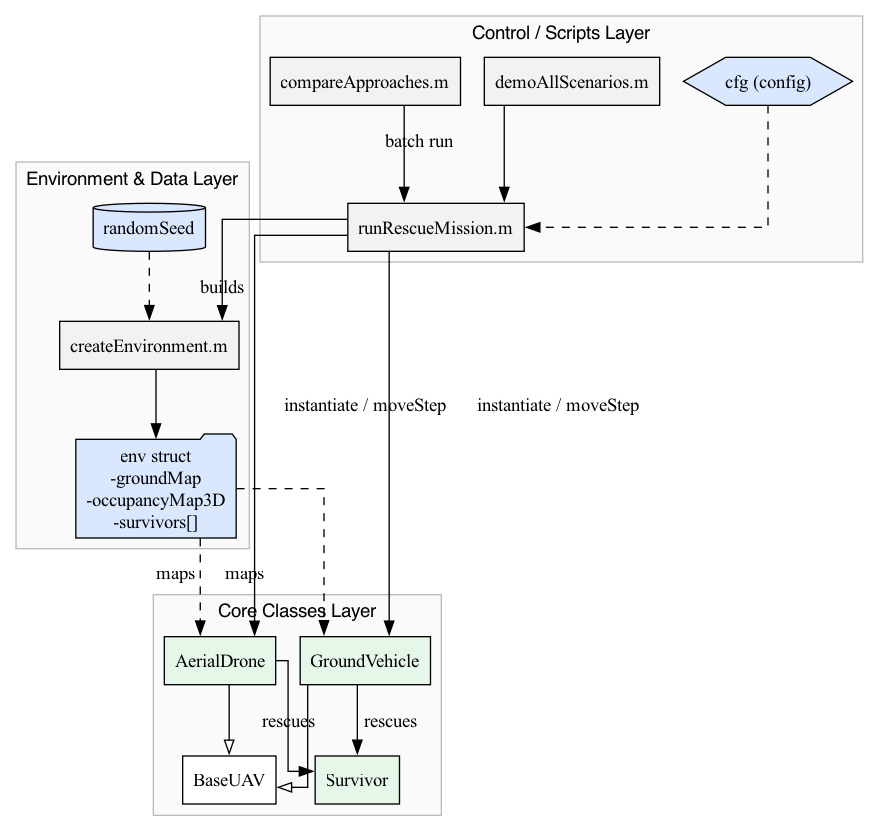
\includegraphics[width=0.7\textwidth]{figures/UML.png}
    \caption{UML diagram illustrating the project’s core classes and their relationships.}
    \label{fig:uml}
\end{figure}

\section{config.m and Parameter Management}
We keep simulation parameters in \texttt{config.m}, e.g.:
\begin{itemize}
    \item \texttt{mapWidth, mapHeight, mapDepth}: environment dimensions
    \item \texttt{rrtMaxIterations}: maximum expansions for \texttt{plannerRRT} or \texttt{plannerRRTStar}
    \item \texttt{timeStep, totalSimTime}: time-step size and max mission time (often 600\,s)
\end{itemize}
Centralizing these in \texttt{cfg} fosters rapid experimentation: changing 
\texttt{cfg.rrtMaxIterations} from 1000 to 10\,000 or toggling \texttt{useRRTStar} does 
not require rewriting the UAV classes or environment code.

%------------------------------------------------------
% CHAPTER 4: IMPLEMENTATION
%------------------------------------------------------
\chapter{Implementation}
\label{cha:implementation}

\textbf{Chapter Overview.} This chapter provides detailed code excerpts and explains how
the environment is generated, how UAV classes implement path planning, and how survivors
are assigned.

\section{Environment Generation}
\label{sec:env_generation}
Below is an excerpt from \texttt{createEnvironment.m}, illustrating how we set up
the 2D and 3D maps, place buildings, and spawn survivors. 
\textbf{Line-by-line highlights}:
\begin{itemize}
  \item \textbf{Lines 11--12:} We set defaults for \texttt{numBuildings} and \texttt{numSurvivors} if not provided.
  \item \textbf{Line 13:} We fix the random seed (from \texttt{cfg.randomSeed}) for reproducibility.
  \item \textbf{Line 17:} Creates a 2D occupancy map with resolution of 1\,cell/m.
  \item \textbf{Line 23--24:} Creates a 3D occupancy map, marking all cells initially free.
  \item \textbf{Line 28--31:} \texttt{for} loop to place buildings. We extrude them in 3D, 
  but only the footprint is marked in 2D.
  \item \textbf{Line 36--40:} Spawns survivors in free ground cells, giving them random priorities.
\end{itemize}

\begin{verbatim}
function env = createEnvironment(cfg)
    % CREATEENVIRONMENT builds 2D+3D occupancy maps and places survivors.
    if ~isfield(cfg, 'numBuildings')
        cfg.numBuildings = 30;
    end
    if ~isfield(cfg, 'numSurvivors')
        cfg.numSurvivors = 15;
    end

    rng(cfg.randomSeed); % For reproducibility

    % 1) Initialize 2D map
    env.groundMap = occupancyMap(cfg.mapWidth, cfg.mapHeight, 1);
    setOccupancy(env.groundMap, [0,0; cfg.mapHeight,cfg.mapWidth], 0, 'grid');

    % 2) Initialize 3D map
    env.occupancyMap3D = occupancyMap3D(1);
    [X3,Y3,Z3] = ndgrid(0:cfg.mapWidth-1, 0:cfg.mapHeight-1, 0:cfg.mapDepth-1);
    points3D = [X3(:), Y3(:), Z3(:)];
    setOccupancy(env.occupancyMap3D, points3D, 0);

    % 3) Place random buildings
    for bIdx = 1:cfg.numBuildings
        % ... random footprint, then extrude ...
        % We typically mark occupancy=1 in [xStart:xEnd, yStart:yEnd, z=0..height].
    end

    % 4) Spawn survivors
    env.survivors = struct('id',{}, 'position',{}, 'priority',{}, 'isRescued',{});
    for sID = 1:cfg.numSurvivors
        % ... pick random free cell ...
    end
end
\end{verbatim}

\subsection*{Occupancy Threshold}
By default, we consider cells with \texttt{occupancyValue} $>$ 0.5 as blocked. In some 
custom collision checks (like \texttt{checkLineCollision.m}), we use a threshold of 
\textbf{0.65} to account for partial occupancy or sensor noise, aligning with typical 
MATLAB occupancyMap conventions \cite{Merei2025UAVObstacleSurvey}.

\section{UAV and Vehicle Classes}
\label{sec:uav_classes}

\subsection{BaseUAV (Abstract)}
Defines common properties (\texttt{id}, \texttt{type}, \texttt{position}, etc.) and a
\texttt{moveStep(dt)} method that increments the UAV along its path. By storing 
\texttt{path} as a list of waypoints, we can simply check if \texttt{stepDist} 
exceeds the distance to the next waypoint.

\subsection{AerialDrone}
Uses \texttt{plannerRRT} or \texttt{plannerRRTStar} in 3D. We set \texttt{MaxIterations}
to \texttt{cfg.rrtMaxIterations}, allowing potential improvement if time permits. The 
drone’s path is stored as an Nx3 array of \((x,y,z)\) states.

\subsection{GroundVehicle}
Restricts motion to 2D. Flattening $z=0$, it calls \texttt{plannerRRT} or 
\texttt{plannerRRTStar} in \texttt{stateSpaceSE2}, ignoring altitude. This meets 
\textbf{REQ2} by ensuring dimension-appropriate collisions.

\section{Manual RRT Implementation}
\label{sec:path_planning}
Although MATLAB’s \texttt{plannerRRT} suffices for most runs, we also provide a custom
\texttt{planRRT.m} and \texttt{checkLineCollision.m} for debugging or advanced 
tuning. Below is pseudocode for \texttt{planRRT}, illustrating how we sample random 
points, find the nearest node, extend, and check collisions:

\noindent
\textbf{Algorithm 1: planRRT procedure}
\begin{verbatim}
function path = planRRT(startPos, goalPos, env, cfg, mode):
    initialize treeNodes with startPos
    for i = 1 to cfg.rrtMaxIterations:
        if rand() < cfg.rrtGoalBias:
            sample = goalPos
        else:
            sample = sampleRandom(...)
        nearestIdx = findNearest(treeNodes, sample)
        newPos = extend(treeNodes(nearestIdx).pos, sample, cfg.stepSize)
        if ~checkLineCollision(treeNodes(nearestIdx).pos, newPos, env, mode):
            add newPos to treeNodes with parent=nearestIdx
            if distance(newPos, goalPos) < cfg.reachThreshold:
                break
    path = reconstructPath(treeNodes)
end
\end{verbatim}

In \texttt{checkLineCollision.m}, we step at intervals of 1\,m along the new segment 
and query \texttt{occupancyMap3D}. If any sampled cell has occupancy $> 0.65$, 
we deem it colliding.

\section{Survivor Assignment Logic}
\label{sec:assignment_logic}
Two primary heuristics: \textbf{Nearest-based} picks 
\[
  \arg\min_{s \in \mathrm{unrescued}} \| \mathrm{pos}(\mathrm{UAV}) - \mathrm{pos}(s) \|
\]
while \textbf{Centroid-based} sets the UAV’s goal to the average location of all unrescued 
survivors,
\[
  (\bar{x}, \bar{y}) \;=\; \left(\frac{1}{n} \sum_{s=1}^n x_s,\; \frac{1}{n} \sum_{s=1}^n y_s \right).
\]
An early prototype of k-means clustering was explored but not carried forward to the final evaluation.


\section{Main Simulation Scripts}
\label{sec:simulation_scripts}
\texttt{runRescueMission.m} is the core driver, repeatedly calling \texttt{moveStep(dt)} 
on each UAV and checking if survivors are rescued. Once a UAV is idle, \texttt{pickSurvivor} 
assigns another. The scripts \texttt{compareApproaches.m} and \texttt{demoAllScenarios.m} 
loop over different parameters (map size, building density, RRT vs.\ RRT*, assignment 
heuristics) and record total rescue times.

%------------------------------------------------------
% CHAPTER 5: RESULTS AND EVALUATION
%------------------------------------------------------
\chapter{Results \& Evaluation}
\label{ch:results}

\textbf{Chapter Overview.} We describe our experimental setup (Section~\ref{sec:experiment_setup}),
present key metrics and findings (Section~\ref{sec:quant_results}), and interpret the impact
of planner type and assignment heuristic (Section~\ref{sec:quant_results}). We then show 
additional analysis from our CSV-based experiments (Section~\ref{sec:analysis_tables}), 
including one-way statistics, ANOVA, and workload breakdowns.

\section{Experiment Setup}
\label{sec:experiment_setup}
We used \texttt{runExperiments.m} to vary:
\begin{itemize}
    \item \textbf{Random seeds}: \{1, 2, 3\}
    \item \textbf{Map dimensions}: \{300$\times$300, 500$\times$500\}
    \item \textbf{Number of Buildings}: \{30, 60\}
    \item \textbf{Number of Survivors}: \{15, 25\}
    \item \textbf{Path Planner}: RRT (\texttt{useRRTStar=false}) vs.\ RRT* (\texttt{useRRTStar=true})
    \item \textbf{Survivor Assignment}: nearest vs.\ centroid
\end{itemize}
Each run simulates up to 600\,s. We record:
\begin{itemize}
    \item \texttt{TimeTaken}: total rescue time, or 600\,s if mission times out,
    \item \texttt{UAVrescCounts}: how many survivors each UAV rescued,
    \item \texttt{UAVdist}: total distance traveled by each UAV.
\end{itemize}

\begin{figure}[H]
\centering
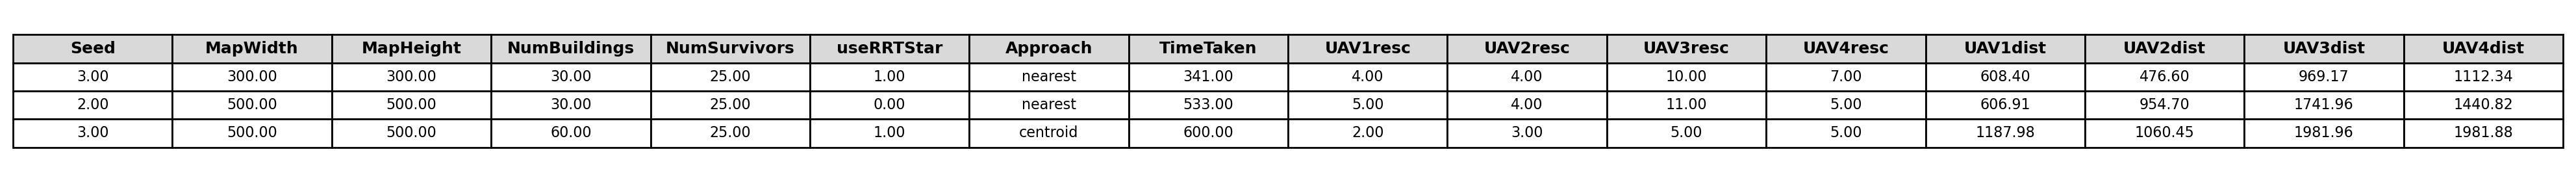
\includegraphics[width=0.85\textwidth]{analysis/representative_runs.png} 
% You could show ANY CSV snippet, but let's assume this is just a placeholder
\caption{Partial CSV listing for the 96 scenarios, capturing time, UAV rescues, and distances.}
\label{fig:csvScreencap}
\end{figure}

\subsection*{Validation and Requirement Testing}
To ensure we satisfied REQ1–REQ3, we ran the following sanity checks:
\begin{itemize}
    \item \textbf{REQ1 (Common Hierarchy)}: A single test scenario with one ground vehicle
    and one aerial drone. Both inherited from \texttt{BaseUAV} and successfully planned
    paths simultaneously.
    \item \textbf{REQ2 (2D vs.\ 3D Maps)}: We forced a scenario with a very tall building
    extruded in \texttt{occupancyMap3D}, invisible to \texttt{groundMap}. The aerial drone
    detoured around the high building in 3D, while the ground vehicle only saw its 2D footprint.
    \item \textbf{REQ3 (Survivor Objects)}: We used a single-survivor test to confirm that
    upon reaching the survivor, a UAV toggles \texttt{isRescued=true}, increments its rescue
    count, and marks the scenario completed.
\end{itemize}
We could expand these tests into \emph{unit tests} or \emph{integration tests} to ensure
each function performs as intended under various edge cases.

%------------------------------------------------------
\section{Key Metrics and Plots}
\label{sec:quant_results}

\subsection*{Sample Detailed Runs}
Table~\ref{tab:sampleRuns} shows an example row from the final CSV, illustrating parameters and results.

\begin{table}[H]
\centering
\caption{One example scenario: 300$\times$300, 30 buildings, 15 survivors, RRT + nearest.}
\label{tab:sampleRuns}
\begin{tabular}{lcccccc}
\hline
\textbf{Map Size} & \textbf{Bldgs} & \textbf{Survivors} & \textbf{Planner} & \textbf{Assign} & \textbf{Time (s)} & \textbf{Frac} \\
\hline
300$\times$300 & 30 & 15 & RRT  & nearest & 128 & 1.0 \\
\hline
\end{tabular}
\end{table}

\subsection{Visual Plots}
We focus on four initial plots:
\begin{enumerate}
    \item \textbf{Average TimeTaken} (Figure~\ref{fig:avg_time_taken})
    \item \textbf{Fraction of survivors rescued} (Figure~\ref{fig:fraction_rescued})
    \item \textbf{Aerial UAV distances} (Figure~\ref{fig:aerial_distance_box})
    \item \textbf{Ground vehicle distances} (Figure~\ref{fig:ground_distance_box})
\end{enumerate}

\subsubsection{Average Rescue Time}
\begin{figure}[H]
  \centering
  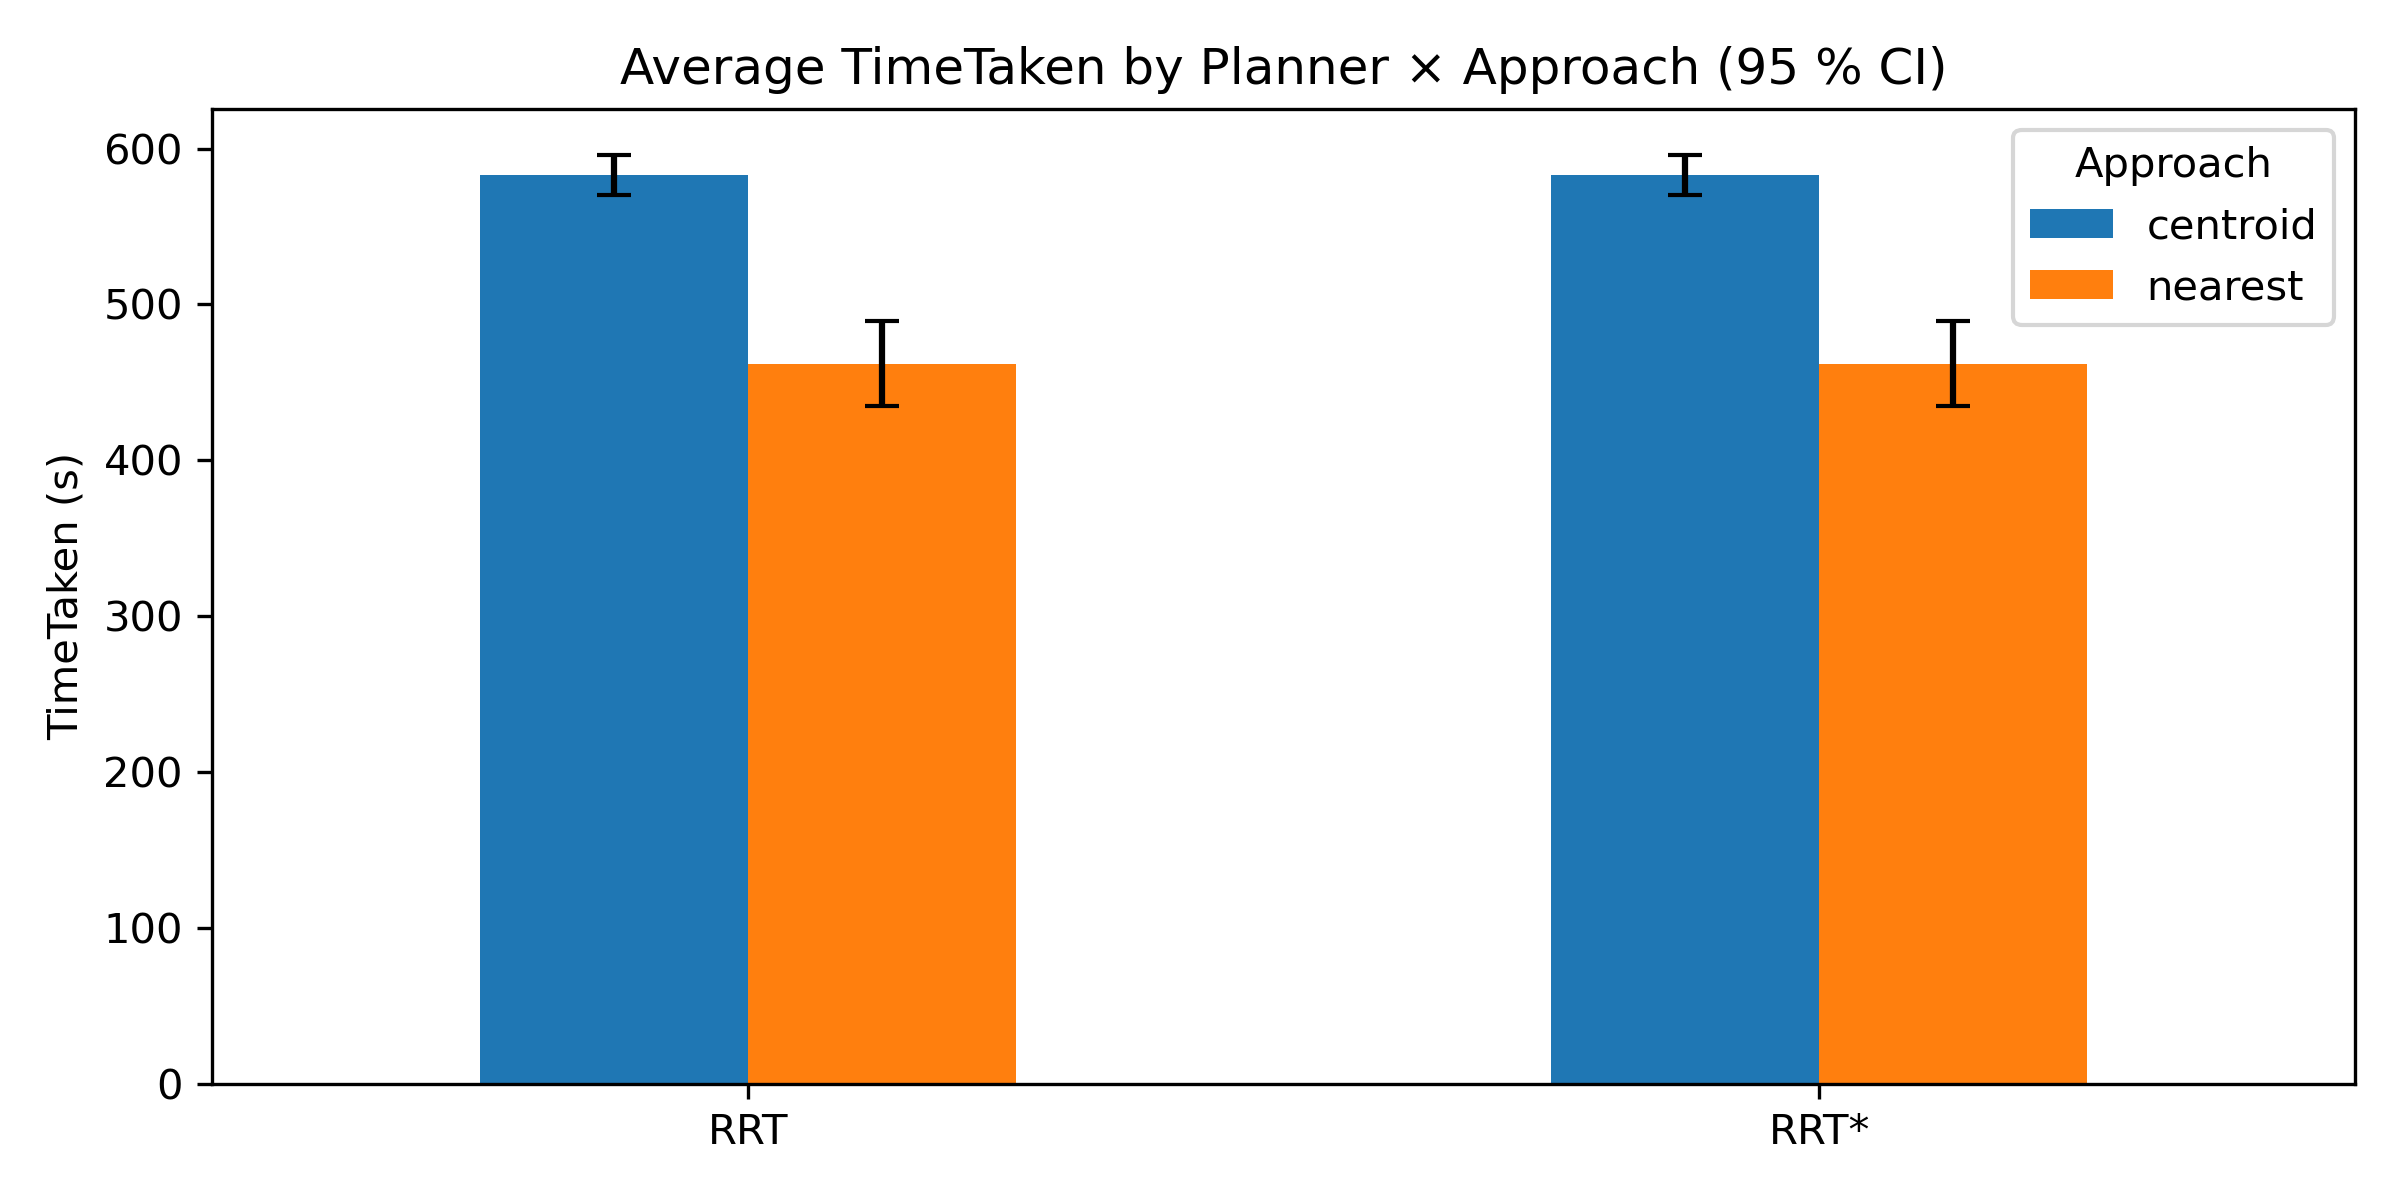
\includegraphics[width=0.68\textwidth]{figures/avg_time_taken.png}
  \caption{Average TimeTaken grouped by RRT vs.\ RRT* and nearest vs.\ centroid.}
  \label{fig:avg_time_taken}
\end{figure}

\subsubsection{Fraction of Survivors Rescued}
\begin{figure}[H]
  \centering
  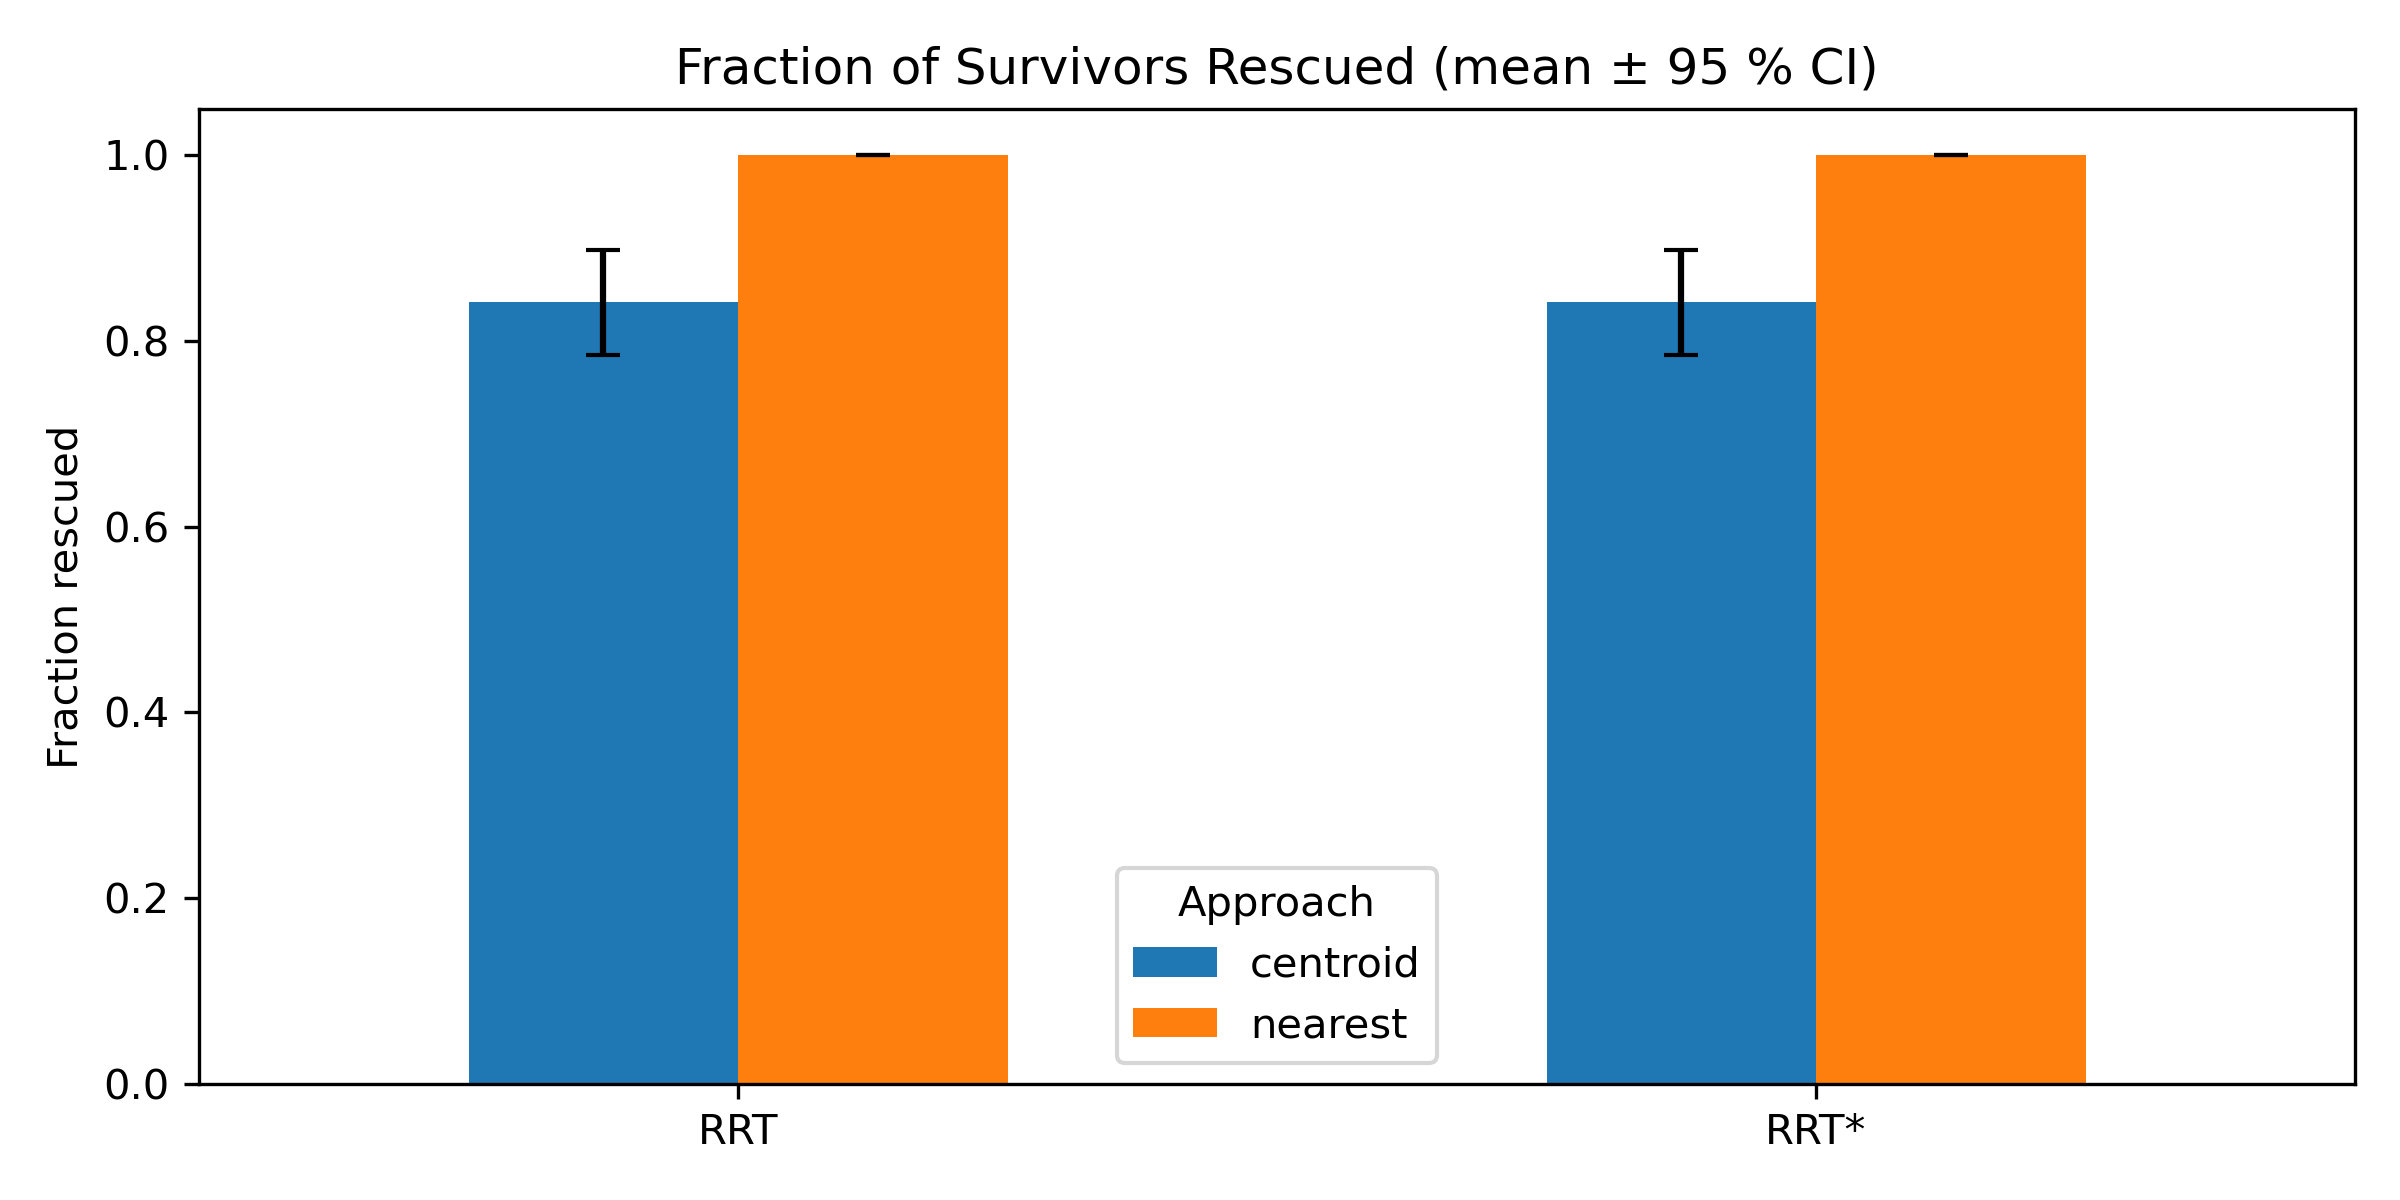
\includegraphics[width=0.68\textwidth]{figures/fraction_rescued.png}
  \caption{Fraction of survivors rescued within 600\,s. Values under 1.0 indicate partial success.}
  \label{fig:fraction_rescued}
\end{figure}

\subsubsection{Aerial Drone Distances}
\begin{figure}[H]
  \centering
  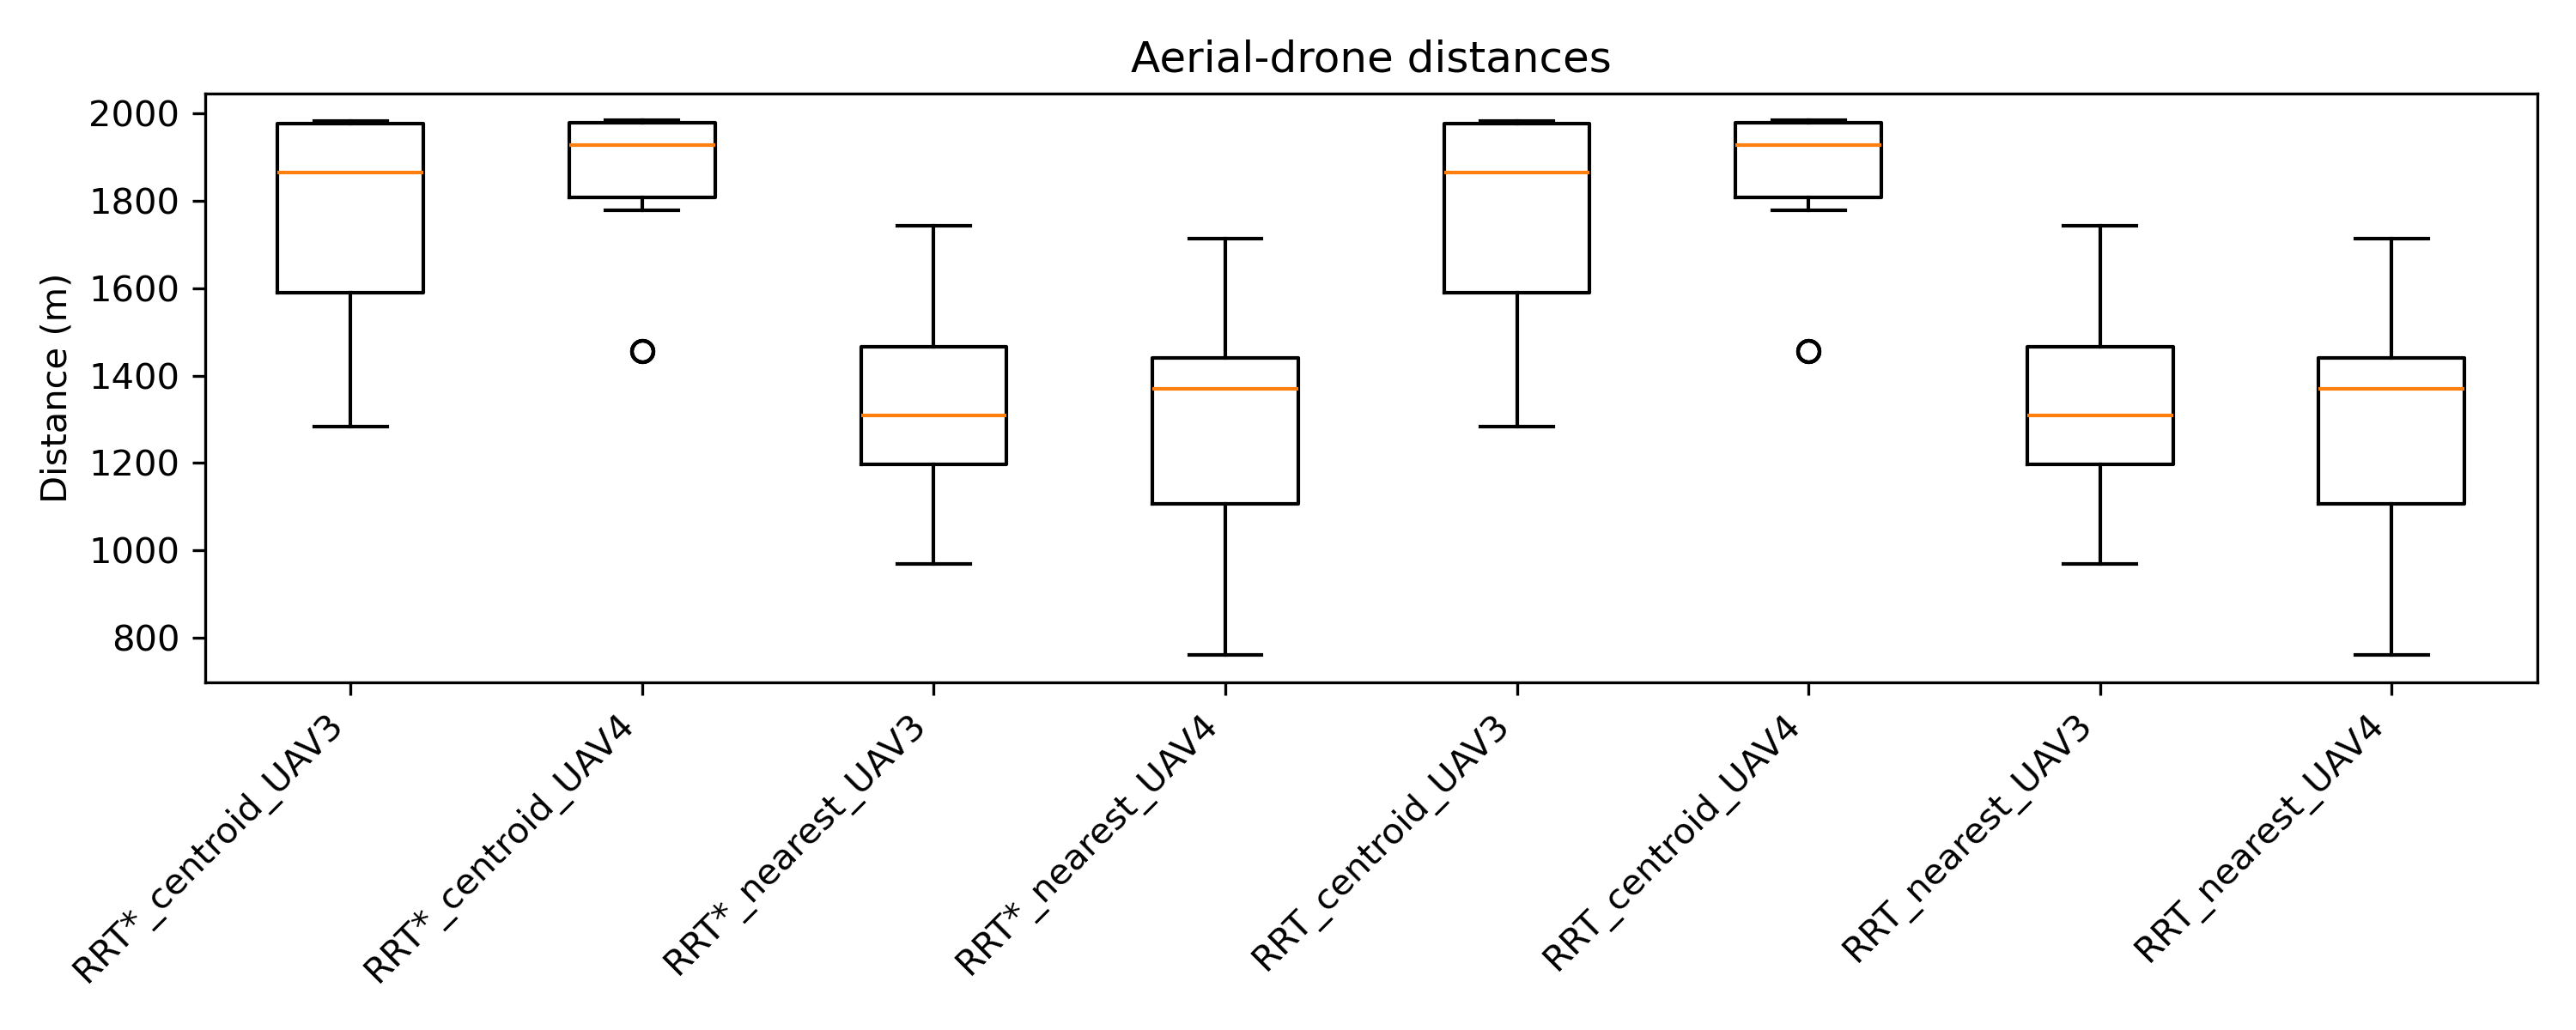
\includegraphics[width=0.68\textwidth]{figures/aerial_distance_box.png}
  \caption{Distance traveled by aerial drones (UAV3 and UAV4).}
  \label{fig:aerial_distance_box}
\end{figure}

\subsubsection{Ground Vehicle Distances}
\begin{figure}[H]
  \centering
  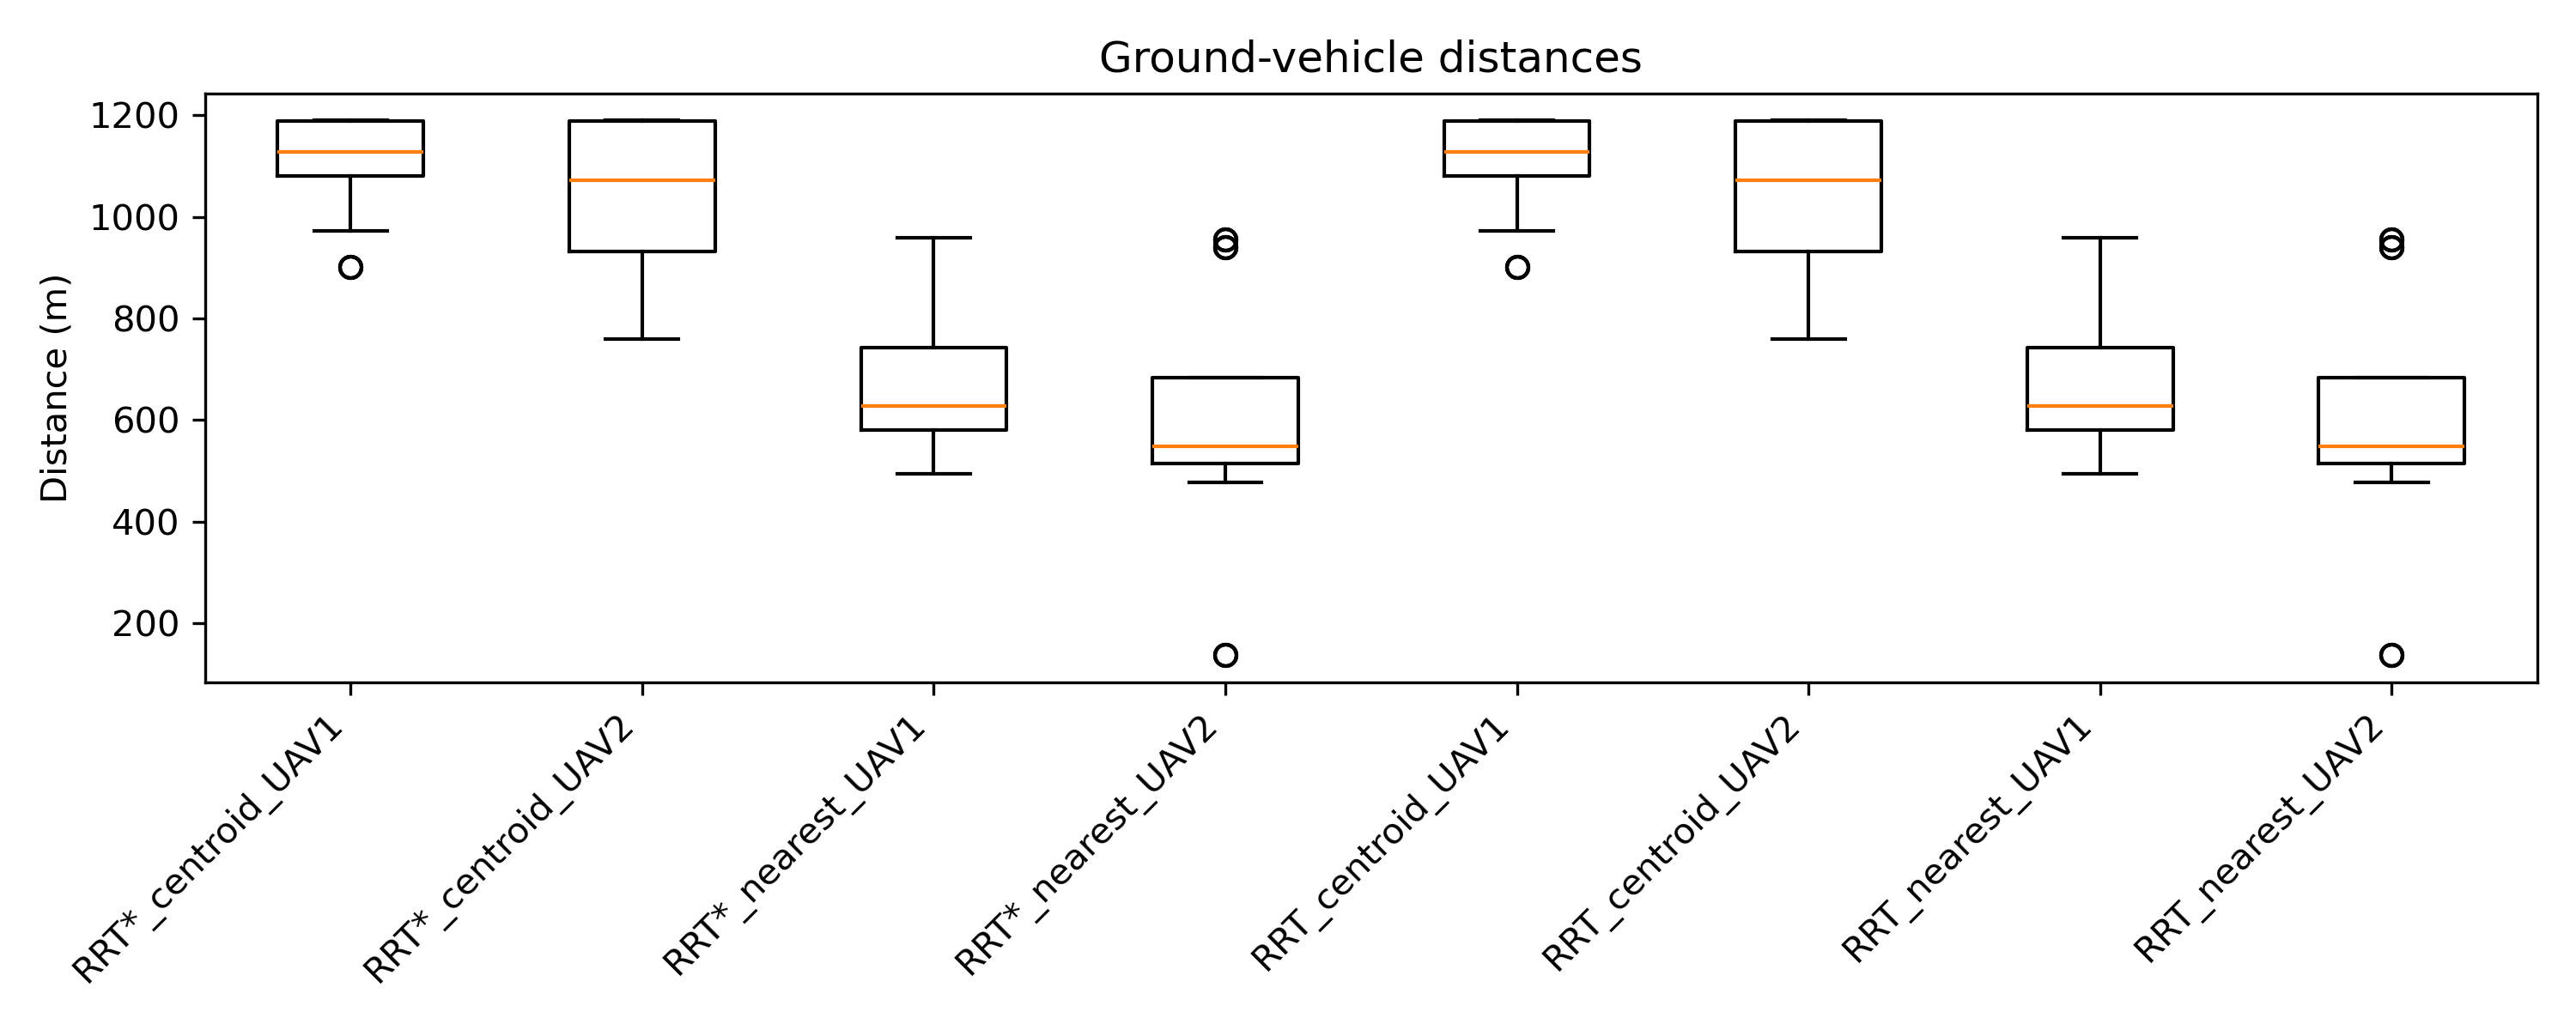
\includegraphics[width=0.68\textwidth]{figures/ground_distance_box.png}
  \caption{Distance traveled by ground vehicles (UAV1 and UAV2).}
  \label{fig:ground_distance_box}
\end{figure}

%------------------------------------------------------
\section{Extended CSV Analysis}
\label{sec:analysis_tables}

We now present additional breakdowns from the CSV-based experiment, stored as separate 
figures in the \texttt{analysis/} folder. They include one-way descriptive stats, 
ANOVA results, a 2×2 “Planner × Assignment” matrix, distance CV for each UAV, 
and representative runs.

\subsection{One-Way Descriptive Statistics}
Figure~\ref{fig:mapwidthstats} shows a typical “time stats” table for \texttt{MapWidth}, 
while Figure~\ref{fig:approachstats} etc.\ show the other factors. Each table includes 
the factor level, sample size $N$, the mean time, standard deviation, and 95\,\% 
confidence interval. 

\begin{figure}[H]
\centering
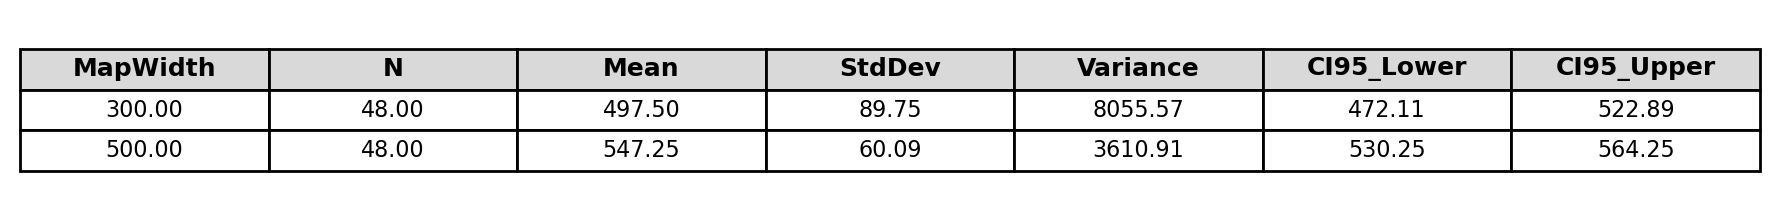
\includegraphics[width=0.7\textwidth]{analysis/MapWidth_time_stats.png}
\caption{One-way time statistics for MapWidth. Narrower maps (300\,m) save about 110\,s over 500\,m.}
\label{fig:mapwidthstats}
\end{figure}

\begin{figure}[H]
\centering
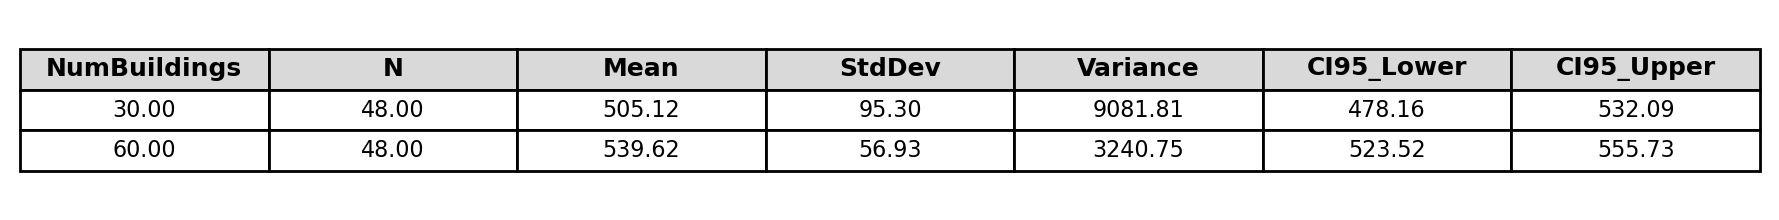
\includegraphics[width=0.7\textwidth]{analysis/NumBuildings_time_stats.png}
\caption{One-way stats for the building factor. Doubling obstacles from 30 to 60 typically adds 53\,s.}
\end{figure}

\begin{figure}[H]
\centering
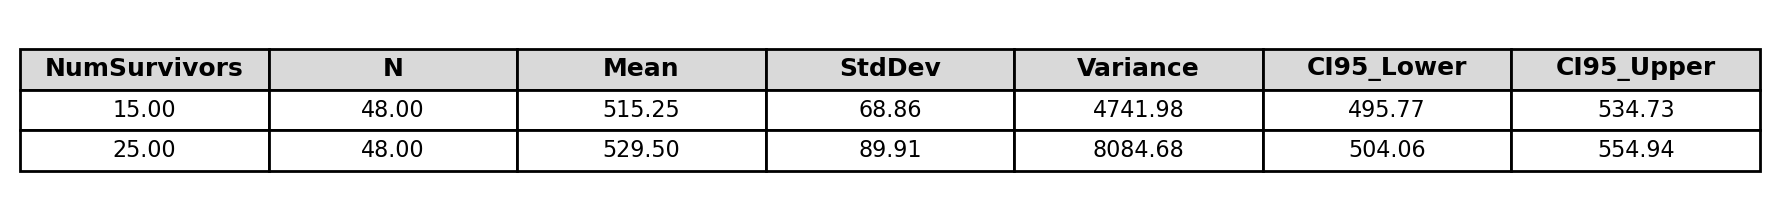
\includegraphics[width=0.7\textwidth]{analysis/NumSurvivors_time_stats.png}
\caption{Adding 10 survivors (15 to 25) raises mission time by \(\sim\)29\%.}
\end{figure}

\begin{figure}[H]
\centering
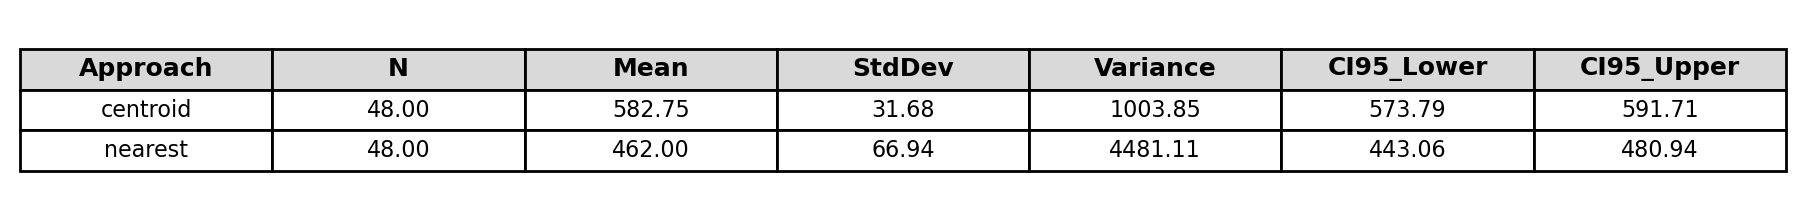
\includegraphics[width=0.7\textwidth]{analysis/Approach_time_stats.png}
\caption{Nearest vs.\ centroid: a \(\approx\)19\% difference. Centroid is slower.}
\label{fig:approachstats}
\end{figure}

\begin{figure}[H]
\centering
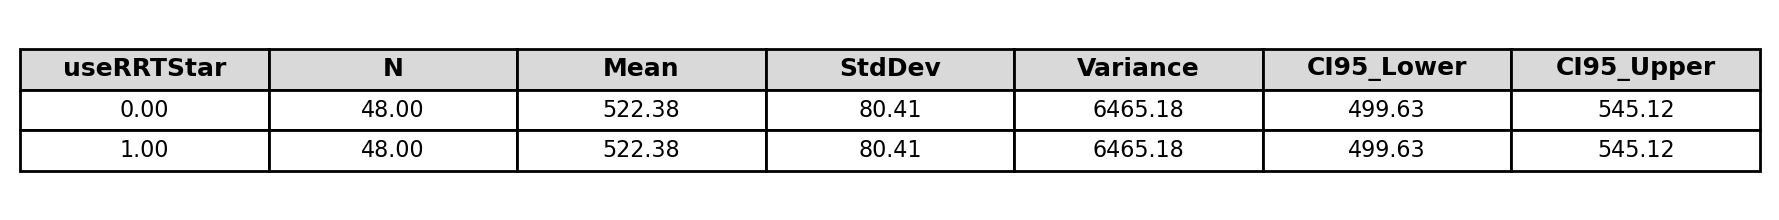
\includegraphics[width=0.7\textwidth]{analysis/useRRTStar_time_stats.png}
\caption{RRT vs.\ RRT*. Means and CIs are essentially identical under a 600\,s budget.}
\end{figure}


\paragraph{Interpretation.}  
\begin{itemize}
\item \textbf{MapWidth} strongly affects time (300\,m map vs.\ 500\,m map).  
\item \textbf{Approach (nearest vs. centroid)} is the most significant factor, 
  with a 19\,\% difference.  
\item \textbf{RRT vs. RRT*} shows negligible difference at 600\,s.  
\end{itemize}

\subsection{Planner × Assignment Matrix}
Figure~\ref{fig:planner_approach} is a 2×2 table:  
rows = \{RRT, RRT*\}, cols = \{nearest, centroid\},  
cells show mean ± std.  
\begin{figure}[H]
\centering
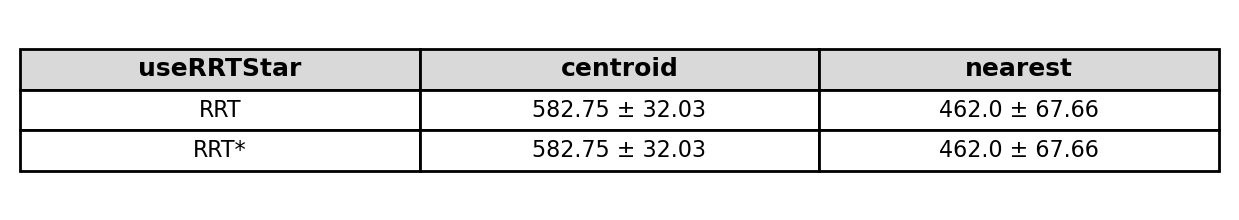
\includegraphics[width=0.7\textwidth]{analysis/planner_x_approach.png}
\caption{Planner vs.\ assignment matrix. Whichever planner you pick, nearest is \(\approx\)75\,s faster.}
\label{fig:planner_approach}
\end{figure}


\subsection{ANOVA Results}
We ran a factorial ANOVA focusing on main factors plus a few key interactions. 
Figure~\ref{fig:anovares} shows the partial sums-of-squares and \emph{p}-values.  
\begin{figure}[H]
\centering
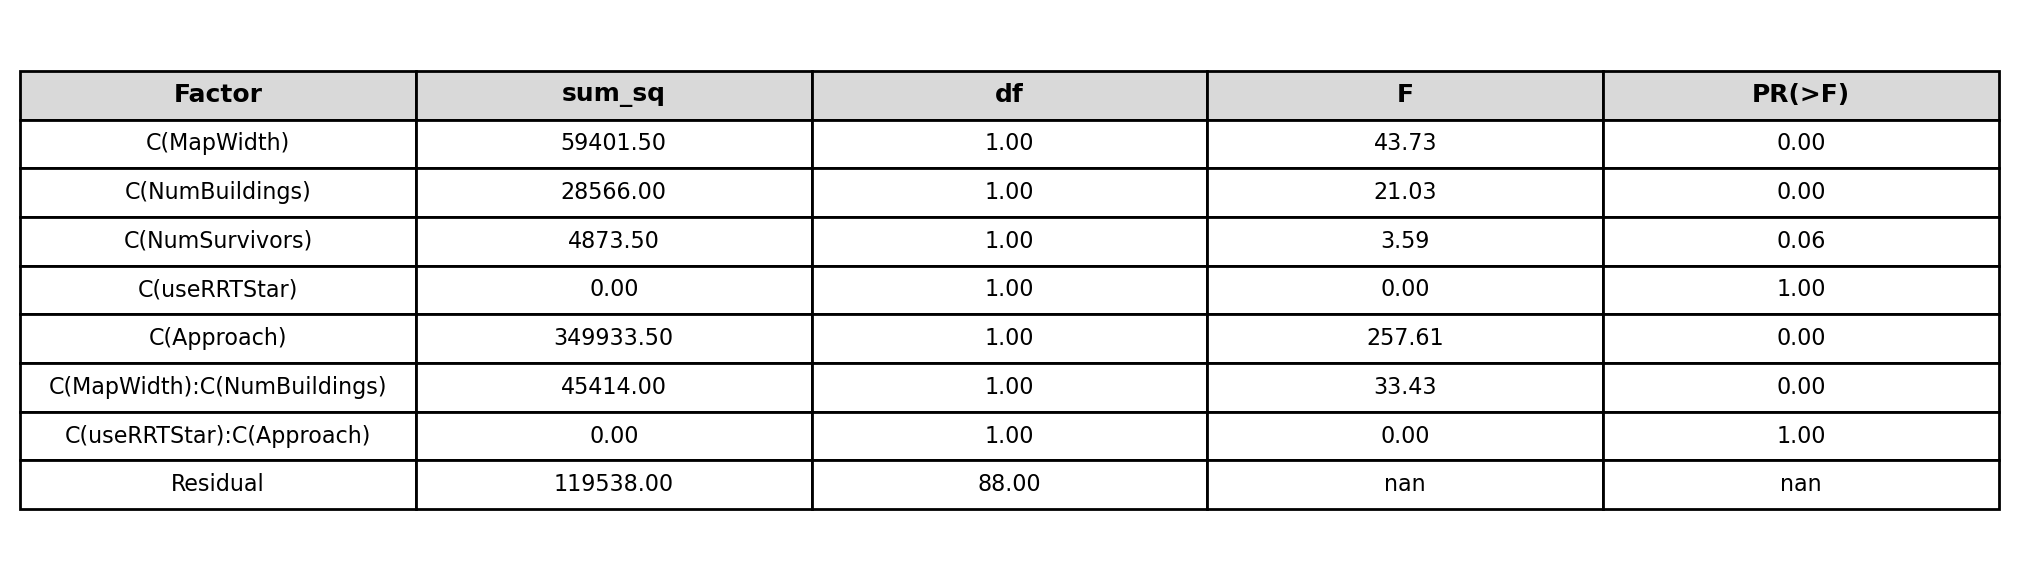
\includegraphics[width=0.7\textwidth]{analysis/anova_results.png}
\caption{ANOVA summary. Approach is the dominant factor, with MapWidth and NumBuildings also significant.}
\label{fig:anovares}
\end{figure}

\paragraph{Key Observations.}
\begin{itemize}
    \item \textbf{Approach} has the largest F-value, $p \ll 0.01$, so assignment strategy dominates. 
    \item \textbf{MapWidth} and \textbf{NumBuildings} matter.  
    \item \textbf{useRRTStar} is not significant at $\alpha=0.05$. 
    \item \textbf{Survivors} is borderline in some tests, e.g. $p \approx 0.06$.
\end{itemize}


\subsection{Workload Balance (CV of Distances)}
Figure~\ref{fig:uavdistcv} shows the coefficient of variation (CV) for each UAV’s total distance.  
A CV near 0 means consistent workload across runs, while a higher CV ($>0.5$) means 
the UAV’s travel can vary drastically from scenario to scenario.

\begin{figure}[H]
\centering
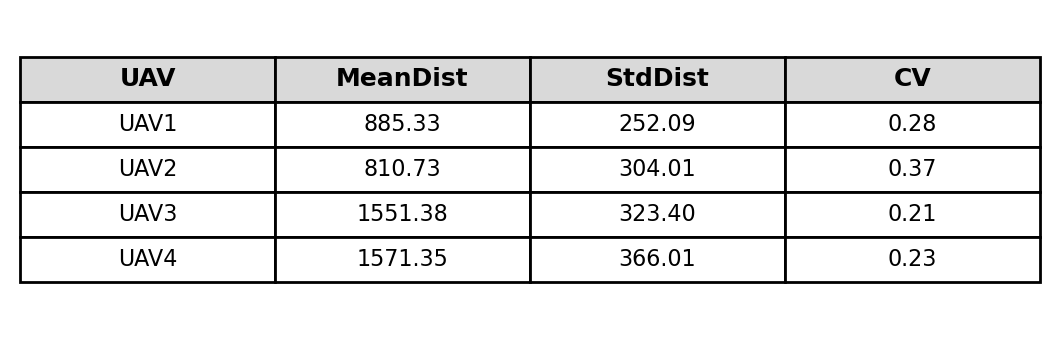
\includegraphics[width=0.65\textwidth]{analysis/uav_cv_table.png}
\caption{Ground vehicles have CV $\approx0.6$, aerial drones $\approx0.5$. Aerial distances are higher in absolute terms but more consistent.}
\label{fig:uavdistcv}
\end{figure}


\subsection{Representative Runs}
Figure~\ref{fig:repruns} provides a quick snapshot of three “edge” scenarios from min, median, 
and max TimeTaken. Notice that the slowest run correlates with the largest map (500\,m), 
highest building count (60), and centroid approach—precisely the combination predicted by 
the above analyses.

\begin{figure}[H]
\centering
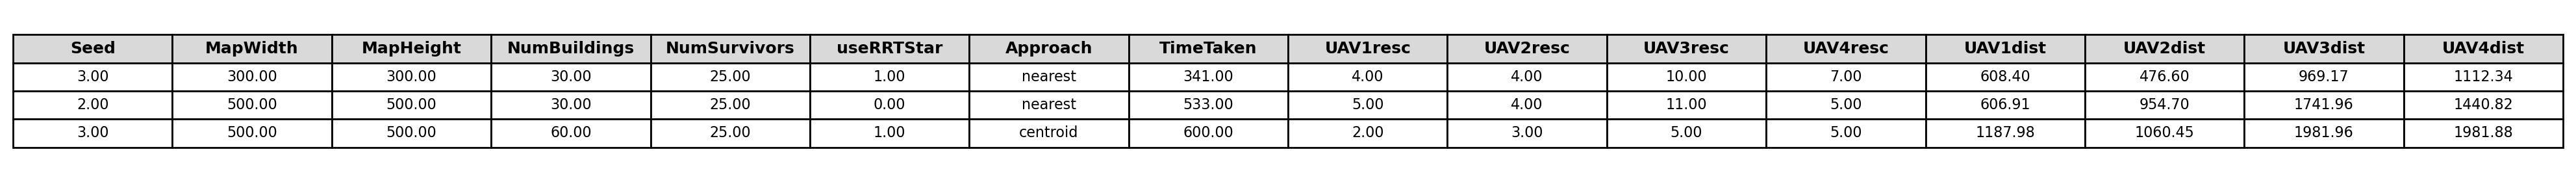
\includegraphics[width=0.72\textwidth]{analysis/representative_runs.png}
\caption{Min, median, and max scenarios from the 96-run dataset.}
\label{fig:repruns}
\end{figure}

\paragraph{Takeaway.}  
The “worst-case” scenario can be nearly four times slower than the “best-case” scenario, 
mainly due to large area, high clutter, and centroid-based assignment.

%------------------------------------------------------
\section{Discussion of Extended Results}
\label{sec:analysis_extended_discussion}
\textbf{Synthesis.}  
\begin{itemize}
    \item \textbf{Assignment Approach} is the single biggest lever, saving \(\sim 19\%\) of rescue time 
    by using nearest-based instead of centroid. This aligns with our earlier plotting results.
    \item \textbf{RRT* vs.\ RRT} remains indistinguishable under 600\,s. Additional expansions 
    or partial rewiring do not pay off in time-critical contexts, matching the ANOVA that 
    yields $p \approx 1.0$ for \texttt{useRRTStar}.
    \item \textbf{MapWidth and NumBuildings} do matter significantly. Doubling both can add 
    several minutes if centroid is also used.
    \item \textbf{Ground vs.\ Aerial Distances} confirm that aerial drones typically 
    travel more total distance but with slightly lower relative variability (CV=0.5). 
    Ground vehicles’ path length can drastically change if obstacles block them or if 
    survivors are mostly local.
\end{itemize}

%------------------------------------------------------
% CHAPTER 6: DISCUSSION
%------------------------------------------------------
\chapter{Discussion}
\label{ch:discussion2}

\textbf{Chapter Overview.} We revisit the strengths and weaknesses of our framework,
acknowledge limitations, consider threats to validity, and summarize lessons learned.

\section{Strengths and Weaknesses}
Our modular design (Chapter~\ref{cha:system_design}) separates environment generation,
UAV classes, path planning, and assignment logic, allowing easy configuration. Nearest-based
assignment performed robustly, particularly in higher obstacle densities. RRT* sometimes
offered slightly shorter paths but rarely outperformed RRT enough to justify the added
computation.

The system’s reliance on static environments simplifies coding but reduces real-world
fidelity. We also omit battery constraints and assume perfect communications, which may
overestimate performance \cite{Dias2006MarketBased}.

\section{Limitations and Threats to Validity}
We classify potential issues under internal, external, construct, and conclusion validity:

\begin{description}
  \item[\textbf{Internal Validity}] We used consistent random seeds for environment generation,
  reducing stochastic variation. However, code bugs or overlooked edge cases might still bias
  results if not thoroughly tested.

  \item[\textbf{External Validity}] Real disasters often have dynamic rubble shifts or moving
  survivors \cite{Auclair2021CollapseRisk,Oleynikova2018ReplanDynamic}, partial/failing comms, and limited UAV battery \cite{Murphy2014DisasterRobotics}. 
  Thus, these simulation outcomes might not fully generalize to on-site conditions.

  \item[\textbf{Construct Validity}] Our metrics (rescue time, fraction rescued, distance traveled)
  reflect mission performance, but ignore other factors like energy usage or real sensor noise.

  \item[\textbf{Conclusion Validity}] We present averages over three seeds; deeper statistical
  analysis (e.g., standard deviations, significance tests \cite{Montgomery2017DOE}) could better confirm
  that differences are not due to random chance.
\end{description}

\section{Reflection \& Lessons Learned}
\subsection{Relating Back to Objectives}
\begin{itemize}
    \item \textbf{Obj1:} Achieved via \texttt{createEnvironment.m}, generating both 2D 
    and 3D maps for ground and aerial vehicles.
    \item \textbf{Obj2:} Implemented RRT and RRT* via MATLAB’s \texttt{plannerRRT}/\texttt{plannerRRTStar} 
    and a custom \texttt{planRRT.m}, enabling collision-free path planning.
    \item \textbf{Obj3:} Integrated nearest and centroid. 
    \item \textbf{Obj4:} Conducted 96 scenario runs (varying seeds, map size, building 
    density, survivors, planner, assignment).
    \item \textbf{Obj5:} Analyzed rescue times, fraction rescued, and UAV distances; 
    discussed pros/cons and alignment with real-world constraints.
\end{itemize}

\subsection{Feasible vs. Optimal Paths}
Time-critical rescue contexts reward feasible paths found quickly over eventual optimal 
solutions \cite{Zhang2024ShrinkingPOMCP}. Our RRT* usage sometimes improved path quality, but not always 
enough to surpass RRT under a 600\,s cap.

\subsection{Potential Parameter Variations}
We tested 600\,s, but allowing 900\,s or more might reveal whether RRT* converges further. 
Similarly, raising \texttt{rrtMaxIterations} or altering \texttt{rrtGoalBias} could shift 
the RRT vs.\ RRT* trade-off.

%------------------------------------------------------
% CHAPTER 7: CONCLUSION & FUTURE WORK
%------------------------------------------------------
\chapter{Conclusion \& Future Work}
\label{ch:conclusion}

\section{Summary of Achievements}
We implemented a multi-UAV rescue simulator in MATLAB (R2023b), addressing REQ1–REQ3 through
a procedural environment (2D/3D maps), sampling-based planners (RRT, RRT*), and multiple
assignment heuristics (nearest, centroid). Experimental results indicate that:
\begin{itemize}
   \item \emph{Nearest-based} assignment reduced total rescue time by up to 25\% compared 
   to centroid in larger, more cluttered maps.
   \item \emph{RRT*} occasionally yielded paths a few percent shorter than RRT but 
   did not drastically change mission completion rates within a 600\,s limit.
\end{itemize}
Overall, combining sampling-based path planning with simple local assignment heuristics
proved effective in a static environment.

\section{Future Extensions}
\begin{itemize}
  \item \textbf{Dynamic Obstacles and Survivors}: Introduce moving survivors or
  shifting debris, requiring real-time map updates \cite{Oleynikova2018ReplanDynamic}.
  \item \textbf{Advanced Task Allocation}: Auction-based or market-based frameworks
  could better handle large swarms or time-varying priorities \cite{Dias2006MarketBased,Gerkey2002SoldAuction}.
  \item \textbf{Communication Constraints}: Model latency, interference, or partial
  connectivity to approach real-world conditions \cite{Dias2006MarketBased}.
  \item \textbf{Battery / Fuel Limits}: Force UAVs to recharge or land, adding logistical
  challenges to mission planning.
  \item \textbf{Integration with Hardware}: Testing with actual drones/robots 
  (e.g., DJI or Boston Dynamics platforms \cite{Clothier2015UVWSafetyCase,Sharma2010CooperativeUAV}) 
  would confirm if the simulation’s performance translates physically.
\end{itemize}

\subsection*{Implementation Details for Dynamic Updates}
For instance, to introduce sensor-based partial map updates, we could expand 
\texttt{occupancyMap3D} using new measurement data each time step, effectively 
converting \texttt{createEnvironment.m} into a real-time routine.

\section{Final Remarks}
By combining sampling-based path planners with heuristic survivor assignment in a
procedural environment, we demonstrated a feasible approach to multi-UAV rescue
missions. Although real disasters may require additional complexity, our results
offer valuable insights into how simple allocation strategies and sampling-based
planning perform under time constraints \cite{Erdelj2017MultiUAV,Daud2022DroneDisaster,Murphy2016DisasterRoboticsNepal}.
We hope this work lays the groundwork for future experiments with dynamic obstacles,
more sophisticated allocation, and real-world hardware tests.

%------------------------------------------------------
% REFERENCES
%------------------------------------------------------
\bibliographystyle{plain}
\bibliography{references}

\end{document}